%% Numbers    checked
%% Spelling   checked
%% Acronyms   checked

\chapter{The Large Hadron Collider}
\label{chap:I-2-lhc}

	The Large Hadron Collider (LHC) \cite{Evans:2008zzb} is a hadron accelerator and collider that is installed in a 26.7 km long tunnel beneath the Franco-Swiwss border near Geneva at a depth varying from 170 m below the Jura mountains to 45 m below the Leman lake. The tunnel was built by the European Organization for Nuclear Research (CERN) between 1984 and 1989 to host the former Large Electron Positron collider (LEP). As represented in Figure \ref{fig:I-2-lhc-schematic} which provides a schematic illustration of the LHC, it is composed of eight arcs, eight straight sections (in between the arcs), and two transfer tunnels which connect the LHC to CERN's main injection complex. From the eight possible collision points located in the straight sections of the tunnel, only four are in use and instrumented with a total of seven particle detectors: ALICE \cite{1748-0221-3-08-S08002}, ATLAS \cite{1748-0221-3-08-S08003}, CMS \cite{1748-0221-3-08-S08004}, LHCb \cite{1748-0221-3-08-S08005}, TOTEM \cite{1748-0221-3-08-S08007}, LHCf \cite{1748-0221-3-08-S08006}, and MoEDAL \cite{Acharya:2014nyr}. \\

	\begin{figure}[h!]
		\centering
		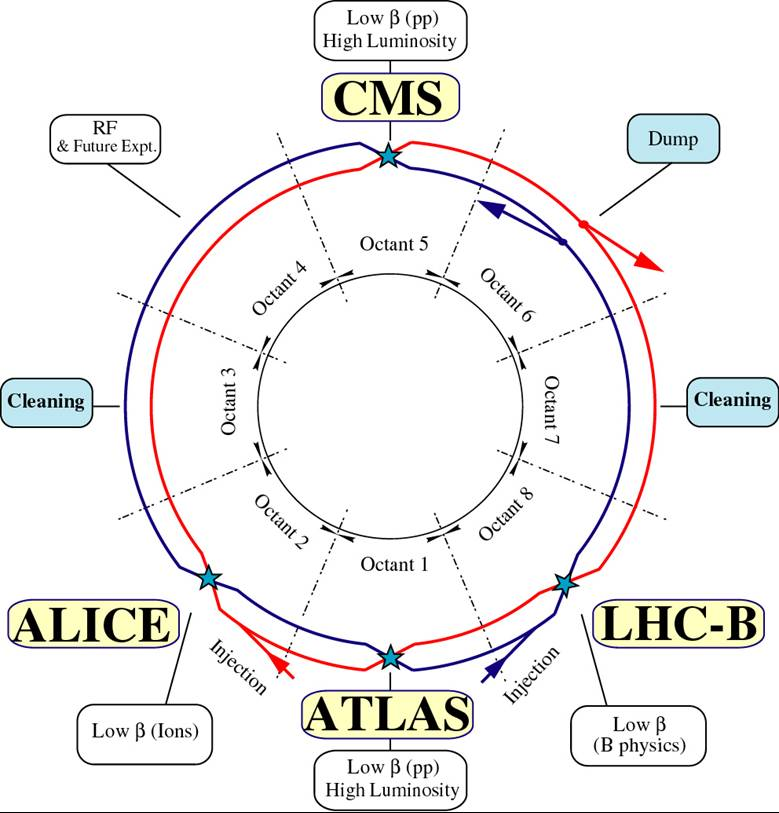
\includegraphics[width=0.7\textwidth]{img/I-2-lhc/lhc.jpg}
		\caption{Schematic representation of the Large Hadron Collider and the four main experiments (ALICE, ATLAS, CMS, and LHCb) that analyze the produced collision \cite{Evans:2008zzb}.}
		\label{fig:I-2-lhc-schematic}
	\end{figure}

  The construction of the LHC, which concept dates back to 1984, was approved by the CERN Council in December 1994 and started in 1998 with the excavation of the caverns that would hold the experimentation sites. In 2003, the first section of the accelerator was assembled inside the tunnel marking the start of the installation phase of the LHC and its detectors, which would span until 2008. On September 10th 2008, the first beam of protons was circulated inside the LHC only to reveal a major technical issue with the superconducting magnets which stopped the machine for nearly a year. In November 2009, reparation works were finished just in time for the LHC to produce its first collisions at 2.36 TeV before a Year-End Technical Stop (YETS), a yearly technical stop during which maintenance is performed on the machine. In February 2010, the LHC restarted with a physics program with collisions at 7 TeV that lasted until February 2013. At that time, the LHC stopped for two years during a Long Shutdown (LS) in order to perform upgrades to prepare it to run at 14 TeV. On June 3rd 2015, the LHC restarted and set a new record with an energy in the center of mass reference frame of 13 TeV.

  \section{The Injection Complex}

    The particles that enter the LHC are first created and accelerated by the injection complex of CERN which network of accelerators is depicted in Figure \ref{fig:I-2-injection-chain}. Protons are extracted from gaseous hydrogen by means of a duoplasmatron, a device that uses a heated filament cathode in conjunction with electric fields to produce electrons that will ionize and break the H$_2$ gas. The resulting protons have an energy of 100 keV and are injected in the Linac2 linear accelerator. \\

		\begin{figure}[h!]
			\centering
			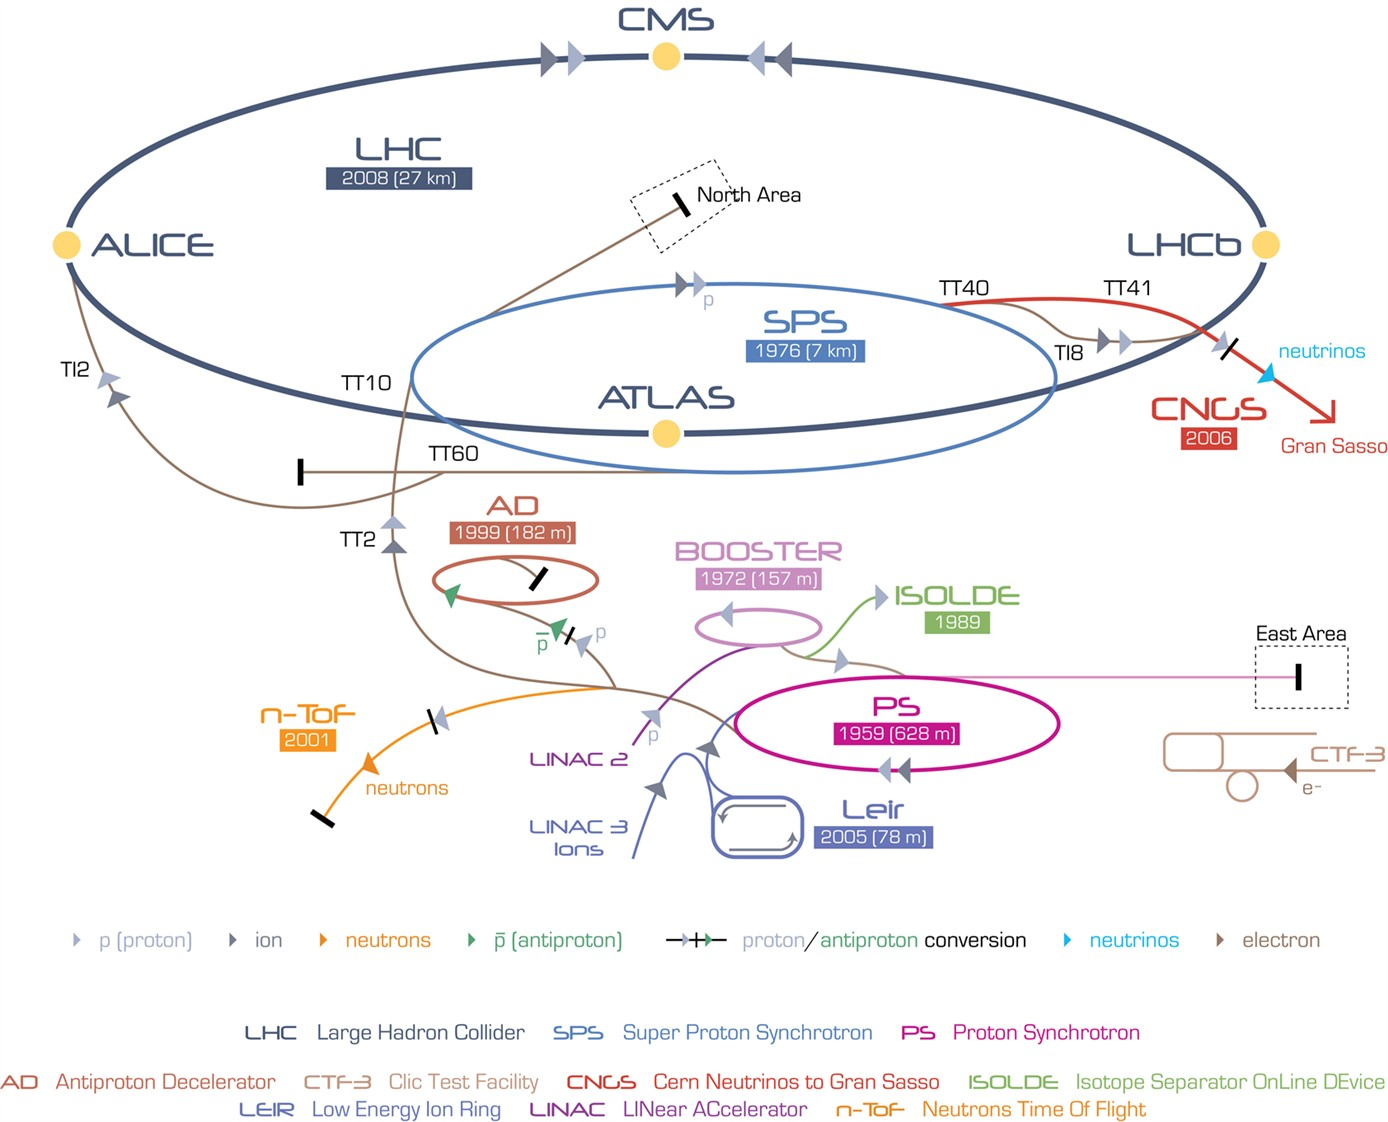
\includegraphics[width=0.9\textwidth]{img/I-2-LHC/injectors.png}
			\caption{Schematic diagram of the injection chain of the LHC composed of multiple smaller accelerators \Cite{TE-EPC-LPC}.}
			\label{fig:I-2-injection-chain}
		\end{figure}

    Linac2 uses radio frequency cavities that produce an electromagnetic field inside the accelerator to transfer energy to the charged particles. The oscillations of the field allow to form bunches of particles by regrouping them on the front of the radio wave. The succession of cavities that form Linac2 boosts the incoming protons to an energy of 50 MeV before they enter the Booster. \\

    Following Linac2, three consecutive circular synchrotrons, namely the Proton Synchrotron Booster (Booster), the Proton Synchrotron (PS), and the Super Proton Synchrotron (SPS), accelerate the beams to energies of respectively 1.4 GeV, 25 GeV, and 450 GeV. Each accelerator is composed of electromagnets that bend the trajectory of the beam and boost it further. From the SPS, the beam is injected in the LHC through two transfer tunnels into two rings where they rotate in opposite directions to be further accelerated until they reach the desired energy. The SPS also provides beam to the North Area were various experiments take place and future technologies can be tested during test beam campaigns frequently organized by CERN.

  \section{LHC Technical Description}

    Once inside the LHC, particles travel through two beam pipes which are subject to a vacuum of 10$^{-10}$ Torr, representing around 3 000 000 molecules per cm$^3$, which greatly reduces the collisions with the air and allow for longer beam longevity. The beam pipes do not form a perfect circle as they are composed of eight arcs and eight straight sections called insertions. \\

    Each arc contains 154 powerful dipole magnets represented in Figure \ref{fig:I-2-magnet} which produce a magnetic field higher than 8 T to bend the beams. The fields are generated by passing high currents through a coil of NbTi superconductor that surrounds the beam pipes cooled by liquid Helium bellow 2 K. The dipoles use a two-in-one design with a common cooling and housing system for the magnets of the two beam pipes which allows to reduce cost and space, and generate a magnetic flux circulating in opposite direction for the two rings. Due to the low temperature at which the magnets operate, the minimum energy deposition left by particles in the coils needed to trigger a quench, a sudden loss of superconductivity, is also decreased. A tight control of the beam structure must thus be enforced. Therefore, 49 quadrupole magnets are installed per section in order to focus the beams and reduce horizontal and vertical spread of the particles. \\

    \begin{figure}[h!]
			\centering
			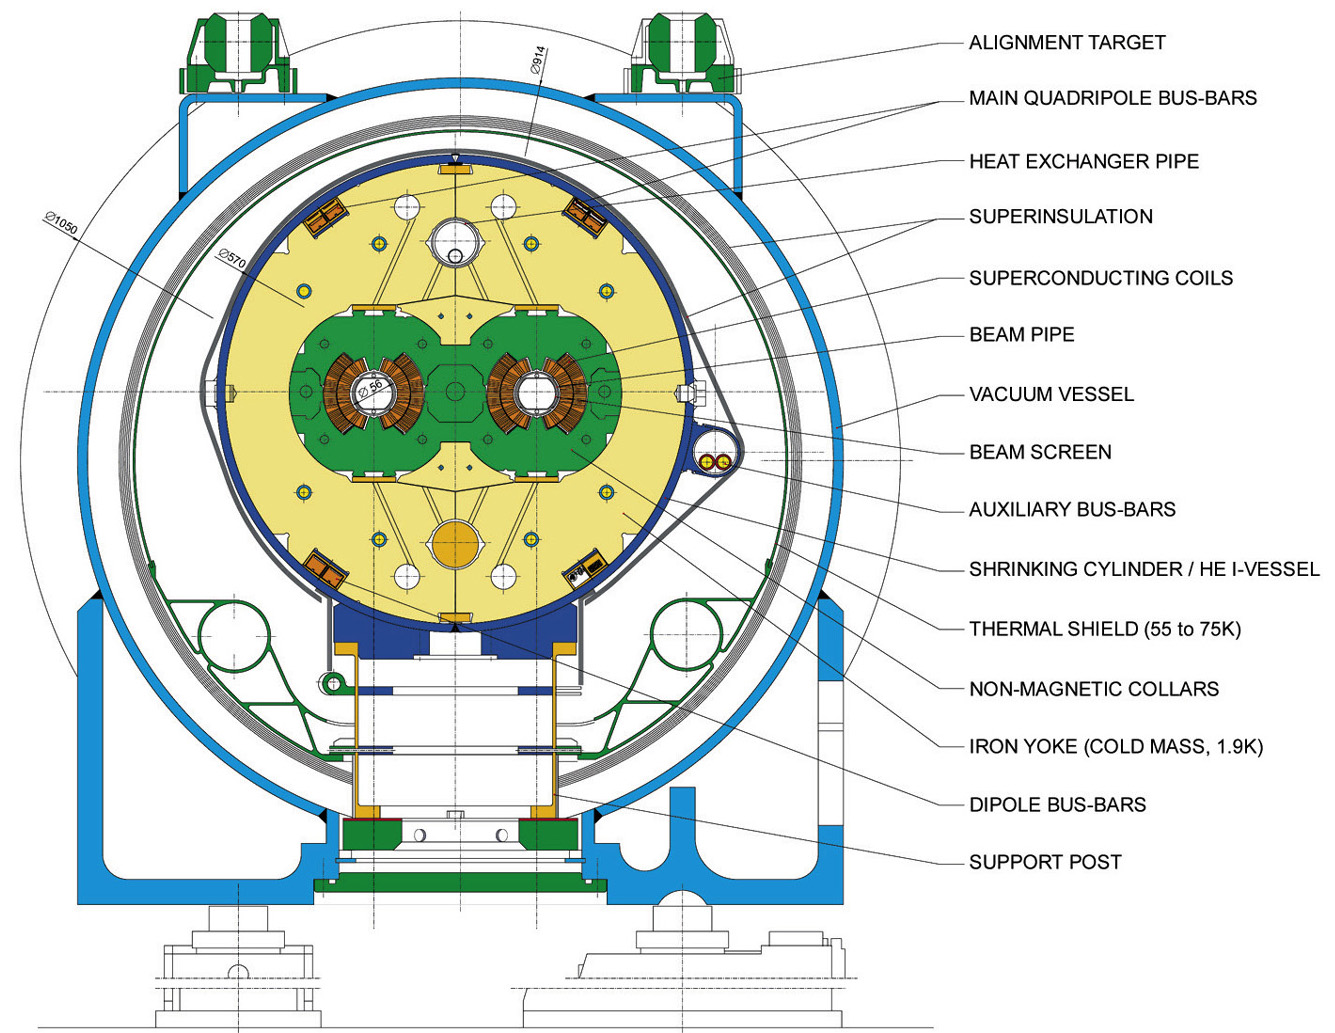
\includegraphics[width=\textwidth]{img/I-2-LHC/magnet.jpg}
			\caption{Cross-section of a cryodipole of the LHC representing the two beam pipes equipped with superconducting NiTb coils surrounded by iron cold mass at 1.9 K \cite{Evans:2008zzb}.}
			\label{fig:I-2-magnet}
		\end{figure}

    The eight straight sections of the LHC have different use cases and designs: four of them are dedicated to the experiments and provide them with collisions, one contains the radio frequency cavities to accelerate the beams, two are use to clean the beam, and one to dump the beam. These functions are fulfilled by using various magnet designs to bend or deflect the beams. From the four collision sites, two also host the beam injection pipes from the SPS into the LHC. The beam cleaning insertions are used to remove particles with out-of-band momentum by scattering them on collimators. When the integrity of the beam is compromised, fast switching magnets activate at the dump insertion in order to quickly extract the particles from the LHC and redirect them to the dump site: an eight meter long graphite composite block that absorbs the energy of the beam.

	\section{Performance Goals}

  	The beams inside the LHC rings are composed of 2808 bunches each made of approximately 110 billion protons. They are separated by 25 ns which is the time between two consecutive bunch crossing (BX), yielding a collision frequency of 40 MHz. During a collision, only a small fraction of the protons interact depending on various parameters such as the crossing angle of the beams, collimation of the bunches, etc. To quantify this, the notion of luminosity has to be introduced and is directly related to the frequency of apparition of events in a given interaction process
  	\begin{equation}
  		f_{process} = \mathcal{L} \sigma_{process} \ ,
  	\end{equation}
  	where $ f_{process} $ is the number of expected events per second, and $ \sigma_{process} $ is the interaction cross-section of the process. For a circular collider, the instantaneous luminosity is defined as
  	\begin{equation}
  		\mathcal{L} = \frac{N^2_b n_b f_{rev} \gamma}{4 \pi \epsilon_n \beta^*} F ,
  	\end{equation}
  	where $ N_b $ is the number of protons or ions per bunch, $ n_b $ is the number of bunches per beam, $ f_{rev} $ is the revolution frequency, $ \gamma $ is the Lorentz factor, $ \epsilon_n $ is the beam emittance, $ \beta^* $ is the beta function at the interaction point, and $ F $ is a function of the crossing angle between the beams. The $ \epsilon_n $ and $ F $ parameters are related to the structure of the bunches and more specifically to their spatial spreading. These parameters change during the operation of the machine as the number of protons per bunch decreases and the bunches spread out. \\

    The instantaneous luminosity can be accumulated over a given period of time in order to obtain the integrated luminosity
  	\begin{equation}
  		L = \int \mathcal{L} \ dt ,
  	\end{equation}
  	which results in the number of events one can expect for a given interaction process
  	\begin{equation}
  		N_{process} = L \sigma_{process} .
  	\end{equation}
    Figure \ref{fig:I-2-luminosity} shows the peak and integrated luminosities delivered by the LHC to its four main experiments during 2015. It can be seen in the picture on the left that the highest instantaneous luminosity reached during that period is on the order of $ 5 \times 10^{33} $ cm$^{-2}$ s$^{-1}$ which is half the nominal luminosity of the current design of the LHC.

		\begin{figure}[h!]
			\centering
			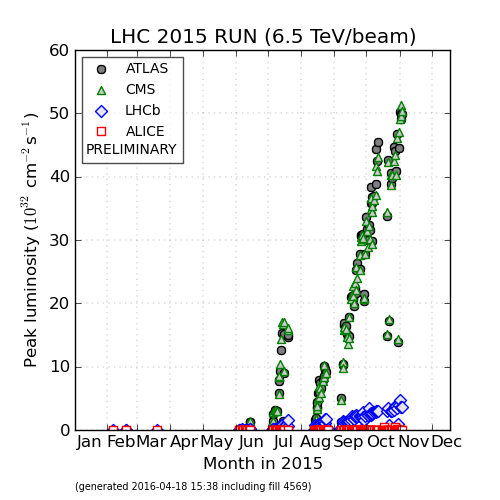
\includegraphics[width=0.49\textwidth]{img/I-2-LHC/luminosity-peak.png}
			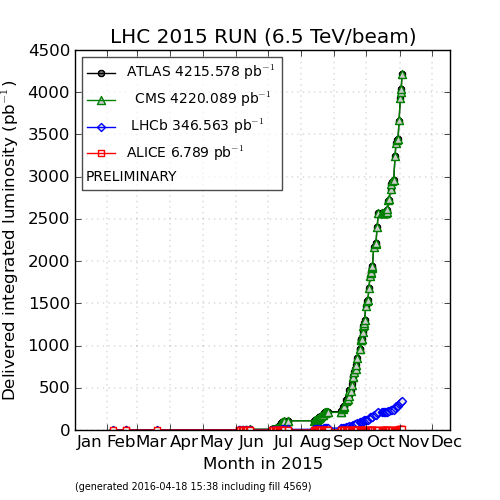
\includegraphics[width=0.49\textwidth]{img/I-2-LHC/luminosity-integrated.png}
			\caption{Monthly evolution of the peak delivered luminosity for the four main experiments of the LHC and the corresponding integrated luminosity \cite{LUMI-PP-LPC}.}
			\label{fig:I-2-luminosity}
		\end{figure}

	\section{Operations and Schedule}

    Over the past years, the LHC has been building up in energy but also in luminosity in order to reach its nominal values of 14 TeV and $ 10^{34} $ cm$^{-2}$ s$^{-1}$. Figure \ref{fig:I-2-futur} depicts the schedule of the LHC for the coming years throughout 2037 and the corresponding luminosities: peak on the left axis and integrated on the right axis. It can be seen that several LS are planned in order to upgrade the LHC and allow the experiments to perform some maintenance and improvements. A noticeable increase in peak luminosity will happen after LS3 and mark the beginning of the so-called Phase2 operation of the LHC. Such an increase in luminosity will affect the experiments due to the higher number of proton-proton collisions during each BX which will in turn translated to a higher flux of particles in the detectors. Preparing the LHC and the detectors to function at such high luminosity is a challenge to which physicists and engineers are already providing answers.

    \begin{figure}[h!]
      \centering
      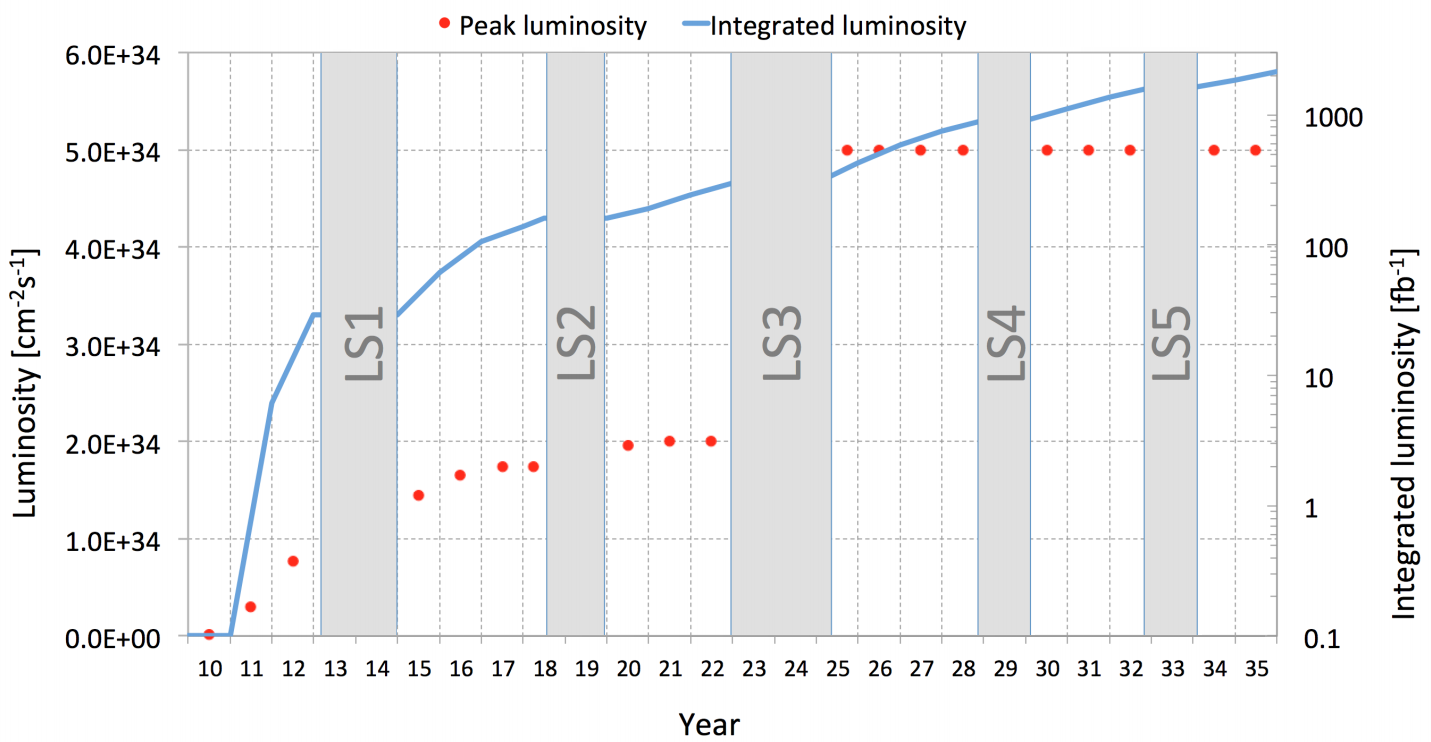
\includegraphics[width=\textwidth]{img/I-2-LHC/lhc-schedule.png}
      \caption{Projected instantaneous and integrated luminosity of the LHC throughout 2037 \cite{HOME-CERN}.}
      \label{fig:I-2-futur}
    \end{figure}

  \section{Scientific Motivations}

    The high energy and luminosity at which the LHC operates are the key factors of its success. Reaching new energy levels enables scientists to discover new hidden sectors of physics as new particles can be created through processes that were previously not able to be generated. Moreover, due to the rarity of these events that lie beyond the Standard Model, it is import to accumulate a large statistics and thus run the machine at high luminosity. \\

    The discovery of the Brout-Englert-Higgs boson is one of the main goals of the LHC which has already been fulfilled. However, the characterization of the particle still requires a great amount of analysis in order to, for example, quantify the coupling constants to fermions or weak bosons. Moreover, it is not excluded that other scalar bosons exist at higher energy as predicted by some theories. In this case, the upgrade of the LHC becomes a necessity to detect the new exotic physics at play. \\

    Not only physics beyond the Standard Model is being explored by the LHC. Measuring the free parameters of the theory and comparing them to theoretical and previously experimentally obtained values is also an important task which helps validating the models. Running at high luminosity allows to study rare processes such as the $ B^0_S $ meson decay, $ \bar{b}s \rightarrow \mu + \bar{\mu} $, which was first observed at the LHC. \\

    The measurements and observations described here above are done by the detectors which are installed on the LHC using the collisions it provides. From the four large experiments the LHC hosts, two of them, namely ATLAS and CMS, are considered to be generalist as they are built to detect a wide range of interactions. ALICE and LHCb on the other hand are optimized to study respectively Pb-Pb interactions at lower energy but which result in a higher density of collisions, and b quark physics to understand the CP violation. The three smaller experiments, namely TOTEM, LHCf, and MoEDAL, use the forward particles that are far away from the interaction point to respectively study elastic collisions, simulate cosmic rays, and search for magnetic monopoles.
